\documentclass[11pt,fleqn]{article}

\setlength {\topmargin} {-.15in}
\setlength {\textheight} {8.6in}

\usepackage{amsmath}
\usepackage{amssymb}
\usepackage{color}
\usepackage{tikz}
\usetikzlibrary{automata,positioning,arrows}
\usepackage{diagbox}



\newcommand{\be}{\begin{enumerate}}
\newcommand{\ee}{\end{enumerate}}

\begin{document}
\begin{center}
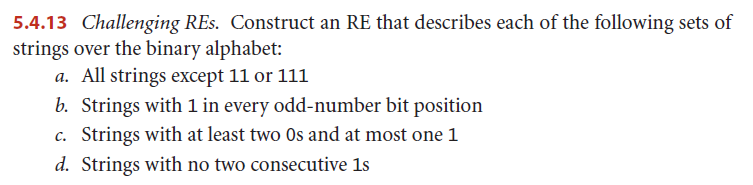
\includegraphics[scale=.8]{5.4.13.png}
\end{center}

\textbf{Solution:}

\be
	\item All strings except 11 or 11: $1|(1^*01|1111(0|1)^*))^*$
	\item Strings with 1 in every odd-number bit position: $(10|11)^*1^*$ OR $1((0|1)1)^*$
	\item Strings with atleast 2 0's and at most one 1: $(1(00)^+|0^+10^+|(00)^+1)$
		\item Strings with no 2 consecutive 1's: $(1(0|01)^*|0(0|01)^*)$ OR $0^*(10^+1)^*0^*$
	
\ee
\end{document}
